\subsection{Ozone mixing ratios as function of NOx and Temperature}

\begin{figure}%
    \centering%
    \caption{Contours of maximum ozone mixing ratio as a function of the total \ce{NO_x} emissions on the first day and daily temperature for each chemical mechanism and using both a temperature-dependent and -independent source of isoprene emissions.}
    \label{f:ozone_contours}%
    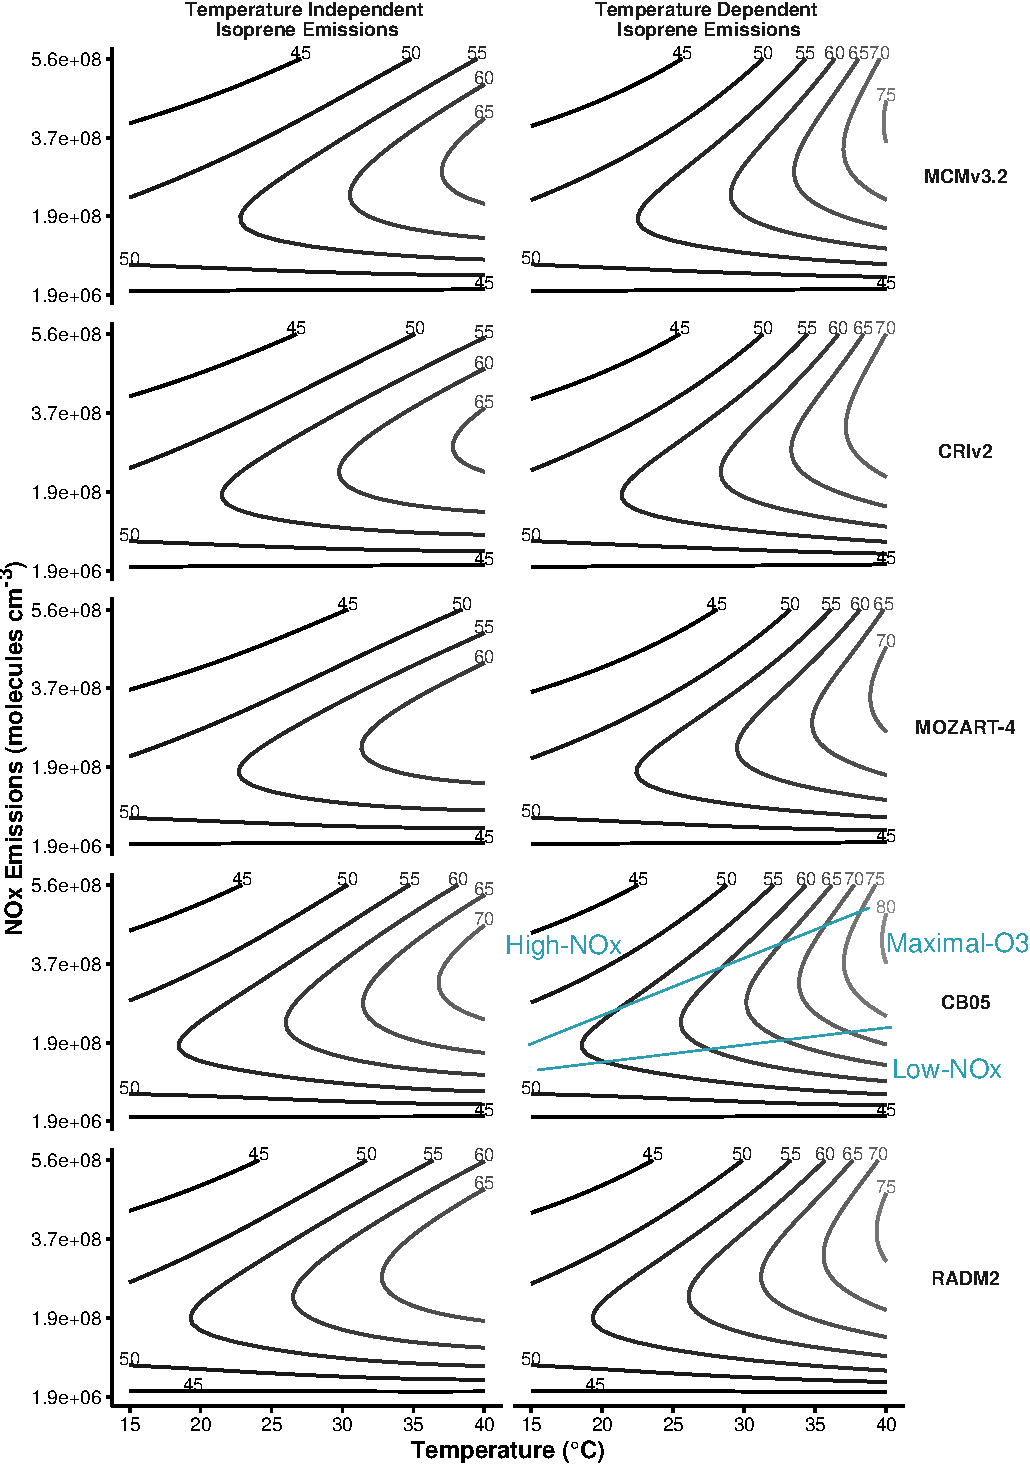
\includegraphics[width=\textwidth]{img/O3_comparison}
\end{figure}

Figure~\ref{f:ozone_contours} depicts the maximum mixing ratio of ozone obtained from each model run as a function of the total \ce{NO_x} emissions on the first day and temperature.
Using each mechanism, a similar non-linear relationship of ozone mixing ratios on \ce{NO_x} and temperature is found and increased ozone levels are found at higher temperatures when including a temperature-dependent source of isoprene emissions.
CB05 and RADM2 produce the largest amount of ozone at higher temperatures than the other chemical mechanisms.
A temperature-dependent source of isoprene, leads to more efficient ozone production \todo{how? prove this} as at higher temperature a lower amount of \ce{NO_x} is required to produce the same amount of ozone as when using a temperature-independent source of isoprene.
At low temperature and high \ce{NO_x}, similar amounts of ozone are predicted from both the temperature-dependent and temperature-independent sources of isoprene emissions.

\subsection{Rate of Change of Ozone with Temperature}

\begin{figure}%
    \centering%
    \caption{Correlation of mean ozone mixing ratio with temperature in Low-NOx, maximal-O3 and High-NOx conditions for each chemical mechanism. A linear relationship between mean ozone mixing ratios and temperature is inferred, regression statistics are found in Table~\ref{t:O3_T_stats}.}
    \label{f:rate_O3_T}%
    \includegraphics[width=\textwidth]{img/Mean_O3_T_NOx_conditions}
\end{figure}

\begin{table}%
    \centering%
    \caption{Regression statistics for the linear relationship between ozone mixing ratios and temperature shown in Figure~\ref{f:rate_O3_T}.}%
    \label{t:O3_T_stats}%
    \scalebox{.78}[.78]{{\renewcommand{\arraystretch}{1.2}
\begin{tabular}{c|c|cc|cc|cc}
	\hline\hline
    \multirow{2}{*}{\textbf{Mechanism}} & \multirow{2}{*}{\textbf{Isoprene Emissions}} & \multicolumn{2}{c|}{\textbf{Low-\chem{NO_x}}} & \multicolumn{2}{c}{\textbf{Maximal-\chem{O_3}}} & \multicolumn{2}{|c}{\textbf{High-\chem{NO_x}}} \\
    & & \textbf{Mixing} & \textbf{No Mixing} & \textbf{Mixing} & \textbf{No Mixing} & \textbf{Mixing} & \textbf{No Mixing} \\
	\hline\hline
	\multirow{2}{*}{MCMv3.2} & Temperature Independent & 0.28 & 1.01 & 0.51 & 1.36 & 0.59 & 0.96 \\ 
    & Temperature Dependent & 0.42 & 1.48 & 0.74 & 2.16 & 0.93 & 2.63 \\ 
	\hline
	\multirow{2}{*}{CRIv2} & Temperature Independent & 0.25 & 0.93 & 0.47 & 1.27 & 0.55 & 0.88 \\ 
    & Temperature Dependent & 0.40 & 1.44 & 0.71 & 2.09 & 0.90 & 2.52 \\ 
	\hline
	\multirow{2}{*}{MOZART-4} & Temperature Independent & 0.25 & 0.97 & 0.44 & 1.21 & 0.49 & 0.59 \\ 
    & Temperature Dependent & 0.38 & 1.43 & 0.65 & 1.98 & 0.81 & 2.05 \\ 
	\hline
	\multirow{2}{*}{CB05} & Temperature Independent & 0.39 & 1.30 & 0.67 & 1.72 & 0.79 & 1.45 \\ 
    & Temperature Dependent & 0.52 & 1.72 & 0.89 & 2.44 & 1.12 & 2.94 \\ 
	\hline
	\multirow{2}{*}{RADM2} & Temperature Independent & 0.37 & 1.31 & 0.61 & 1.64 & 0.70 & 1.28 \\ 
    & Temperature Dependent & 0.48 & 1.68 & 0.79 & 2.22 & 0.97 & 2.49 \\ 
	\hline\hline
\end{tabular}}}

\end{table}
